% ===== PDF p.103 (原书 p.95) =====
% 本章原书节号用阿拉伯数字（1 はじめに、2 …），与全书默认的罗马数字不同；
% 按体例在 \chapter 之前切换编号，章末 reflist 之后恢复。
\renewcommand{\thesection}{\arabic{section}}

\chapter{Floer 同调与镜像对称}
\chapterauthor{深谷賢治}{[京都大学大学院理学研究科]}

\section{引言}

Floer 同调是无穷维空间的同调论。最典型的无穷维空间是环路空间。所谓环路空间 $\Omega M$，就是从圆周 $S^1$ 到空间 $M$ 的映射全体构成的空间。

普通的同调论，例如奇异同调论，对任何拓扑空间都能定义，所以环路空间的同调也可以考虑。环路空间的普通同调群也很重要，自古以来就被深入研究。例如，Morse 提出 Morse 理论的动机，就在于研究闭测地线（从 $S^1$ 出发的映射，把“长度”看作环路空间上的函数时，“长度”在那里取极值的那一类映射）。实际上，利用环路空间同调群的非零元素，就能作出闭测地线。

Floer 同调与“环路空间的普通同调群”不同。简单说明一下二者的差别。空间 $X$ 的一个 $k$ 维同调类，大体上是 $X$ 中包含的 $k$ 维图形（按应有的等价关系考虑所得的等价类）。环路空间的情形也一样：$\Omega M$ 的 $k$ 次同调群，就是 $\Omega M$ 中包含的 $k$ 维图形的等价类。$M$ 是二维球面 $S^2$ 时，情况如下。对所有非负整数 $k$，有
\[ H_k(\Omega S^2;\Q)=\Q. \]
（定义同调时，需要取一个作为系数的环。这里为让答案简单，取了有理数全体 $\Q$。）

给出 $H_0(\Omega S^2;\Q)$ 的元素的 1 维图形，是由 1 点构成的环路。也就是说，例如取北极 $p_0$，考虑只由 $l(t)=p_0$ 这一个环路构成的集合，它就给出 $H_0(\Omega S^2;\Q)$ 的生成元。
% [Tutor Note: 原书此句印作「1 次元の図形」，但由 1 点构成的环路作为图形是 0 维的（正对应 $H_0$），原文此处自相矛盾，疑「1 次元」为「0 次元」之误；译文照原文录。]

$H_1(\Omega S^2;\Q)$ 的生成元更有趣些。它例如由经过 $p_0$、关于经度 0 度的子午线对称的小圆全体构成的图形给出（图 1）。

% ===== PDF p.104 (原书 p.96) =====
\begin{figure}[t]
  \centering
  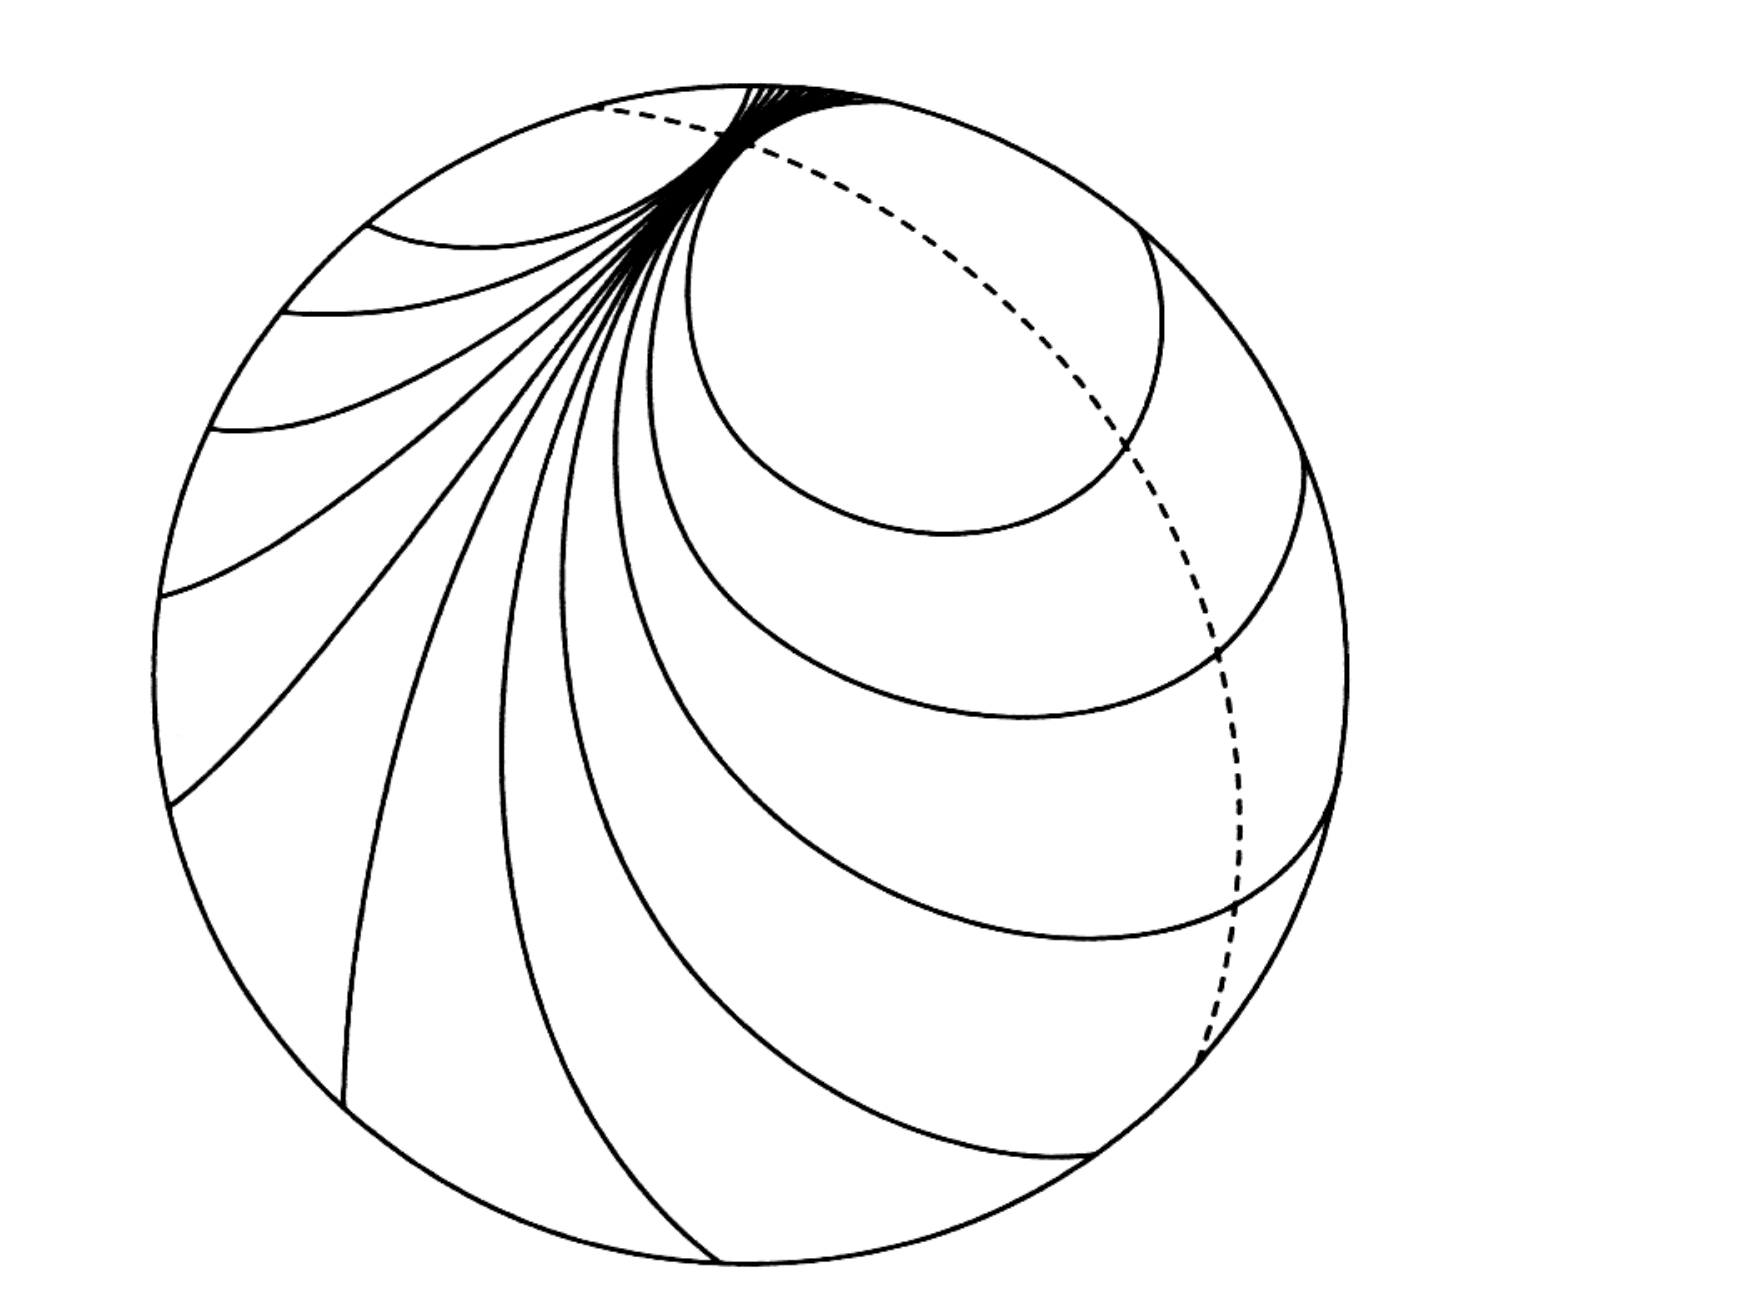
\includegraphics[width=0.74\linewidth]{figures/ch08-fig1.png}
  \figtitle{1}{$H_1(\Omega S^2;\Q)$ 的生成元：经过 $p_0$、关于经度 0 度的子午线对称的小圆族（原书 p.96）}
\end{figure}

这件事与闭测地线有关。也就是说，由 1 点构成的环路作为 $H_0(\Omega S^2;\Q)$ 的元素，是最短的闭测地线。此外，小圆族所代表的 $H_1(\Omega S^2;\Q)$ 的元素之中包含大圆，而大圆是仅次于 1 点的最短闭测地线。

Floer 同调也仍然给出环路空间的同调群，但那是完全不同的同调群。例如，$S^2$ 的环路空间的 Floer 同调是
\[ HF_*(S^2;\Q)\cong H_*(S^2;\Q), \]
也就是说，只有 0 次和 2 次是 $\Q$，其余全部为 0。（这里写成了 $HF(S^2)$。$M$ 的“环路空间的 Floer 同调”习惯上写作 $HF(M)$。$F$ 是创始人 Floer 的首字母。）

这样一来，Floer 同调与普通同调就变得大不相同。其理由是：Floer 同调是
\begin{center}
\textbf{半无穷维}
\end{center}
的同调论。用记号写出来就是，
\[ HF_k(M)=H_{k+\frac{\infty}{2}}(\Omega(M)). \]

% ===== PDF p.105 (原书 p.97) =====
也就是说，所谓 Floer 同调，就是“考虑环路空间中半无穷维的图形，再取其应有的等价类”所得的东西。

这样写，“半无穷维的图形”究竟是什么，立刻就成了问题。现在还不能照这样把“半无穷维的图形”在数学上严格定义，并以其等价类的集合来定义 Floer 同调。尽管如此，Floer 还是设法定义了半无穷维的同调，并找到了它的应用，特别是对变分法的应用。Floer 同调不只在各种环路空间上，在三维流形的联络空间等空间上也能定义，它在规范理论的数学研究等方面也起了很大的作用。

Floer 同调在镜像对称中的作用，一言以蔽之，如下所述。

\begin{center}
\textbf{镜像对称是辛几何与复几何之间的对称性。复流形上以层为系数的上同调论在辛几何中的对应物，就是 Floer 同调。}
\end{center}

高维复几何与代数几何的基础理论大体完成，是在 1950--1960 年代；当时所用的中心工具，就是层及其上同调论。这么一想，读者大概就能明白 Floer 同调在辛几何中的重要性了吧。

上面写的“口号”，与同调镜像对称这一镜像对称的形态密切相关。关于这一点，我想放到第 10 章《镜像对称与同调代数》中说明；本章的主目的，是说明 Floer 同调是什么。

首先，来说明几件似乎与半无穷维有关的事情吧。

\section{狄拉克之海}

最初是 Dirac 的电子论。所谓 Floer 同调与 Dirac 电子论的类比，是从 Witten 在京都的国际数学家大会上的演讲（已经是 15 年以上的事了）那里照搬来的。Dirac 建立了电子在相对论意义下不变的理论。其基本方程即 Dirac 方程
% ===== PDF p.106 (原书 p.98) =====
是 Laplace 方程的平方根一类的方程：Laplace 方程是 2 阶微分方程，而它是 1 阶微分方程。

一个很大的差别在于：Laplace 算子的特征值全部非负，而 Dirac 算子的特征值中，正的与负的各有无穷多个。这样一来，“Dirac 算子的特征函数是电子的状态、特征值就是它的能量”这一解释就出了问题。也就是说，存在负能量状态。对此，Dirac 提出了一种解释：负能量状态早已被填得满满的，所以不会出现。（这称为空穴理论。）无穷多种状态之中，只填满了半数（也就是负的那些全体）的就是真空——这就是他的解释。

换一种说法：普通的状态，是从 $\frac{\infty}{2}$ 次的状态出发只差有限个自由度的状态。这就是 $\frac{\infty}{2}$ 次出现的一个例子\footnote{据说 Dirac 的空穴理论在现今的场论中已被舍弃，但 $\frac{\infty}{2}$ 维这一图像我想还保留着。}。

\section{佐藤 Grassmann 流形}

佐藤幹夫对 KP·KdV 方程有一个重要发现：它是无穷维 Grassmann 流形上的动力系统\footnote{关于佐藤的孤子理论，例如参见 [4]。}。佐藤在那里使用的无穷维 Grassmann 流形，与通常的稍有不同。下面来说明。所谓 Grassmann 流形，就是某个线性空间中固定维数的线性子空间全体。例如，$\C^n$ 中 $k$ 维复线性子空间全体记作 $Gr(n;k)$。在这个类比下，佐藤 Grassmann 流形就是 $Gr(\infty,\frac{\infty}{2})$。

再写得更准确一些。对每个整数 $k\in\Z$，取向量 $e_k$，考虑以无穷多个基 $e_k\ (k=0,-1,1,-2,2,\cdots)$ 构成的向量空间 $V$\footnote{其实需要适当的完备化，这里省略。}。作为它的子空间，考虑只以非负的 $k$ 对应的 $e_k$ 为基的那个，记作 $L_{\ge 0}$。再考虑只以负的 $k$ 为基的那个，记作 $L_{<0}$。二者都可以看作半无穷维的。

% ===== PDF p.107 (原书 p.99) =====
考虑商空间 $V/L_{\ge 0}$，把射影
\[ V \longrightarrow V/L_{\ge 0} \]
记作 $\pi$。$\pi$ 在 $L_{<0}$ 上的限制给出同构
\[ L_{<0}\cong V/L_{\ge 0}. \]
所谓佐藤 Grassmann 流形，就是与 $L_{<0}$“只相差有限个”的子空间全体，其定义如下。

对 $V$ 的线性子空间 $L$，考虑把 $\pi$ 限制在 $L$ 上所得的映射
\[ \pi|_L : L \longrightarrow V/L_{\ge 0}. \]
它的核
\[ \operatorname{Ker}(\pi|_L)=\{v\in L\mid \pi|_L(v)=0\} \]
是有限维的，余核
\[ \operatorname{CoKer}(\pi|_L)=\frac{V/L_{\ge 0}}{\operatorname{Im}(\pi|_L)} \]
也是有限维的，并且
\[ \dim\operatorname{Ker}(\pi|_L)-\operatorname{Coker}(\pi|_L)=0 \]
成立；满足这些条件的 $L$ 的全体，就是佐藤 Grassmann 流形。
% [Tutor Note: 原书此处第二个 $\operatorname{Coker}$ 前似脱 $\dim$，按指标定理应为 $\dim\operatorname{Ker}(\pi|_L)-\dim\operatorname{Coker}(\pi|_L)=0$；且原书 $\operatorname{CoKer}$ 与 $\operatorname{Coker}$ 两处写法混印，此处均照原文录。]

例如，取以 $k<-2$ 的所有 $e_k$ 以及 $e_{-1}+e_0$、$e_3$ 为基的向量空间 $L$。这时，核 $\operatorname{Ker}(\pi|_L)$ 只以 $e_3$ 为基，所以是 1 维；余核 $\operatorname{CoKer}(\pi|_L)$ 只以 $[e_2]$（$e_2$ 的等价类）为基，所以也还是 1 维。

\section{Hamilton 形式与 Lagrange 形式}

前面第 2、3 节讲的内容，请当作铺垫。从这里开始才是正题。学分析力学时会学到两种变分法。一种是 Hamilton 形式，另一种是 Lagrange 形式\footnote{关于第 4、5 节，详见分析力学的书，例如 [1]。}。其中 Lagrange 形式的变分法以第 1 节所述的 Morse 想法为基础，与环路空间的普通同调有关。另一方面，Hamilton 形式的变分法则发展成 Floer 同调。下面来说明这件事。

为简单起见，先考虑 1 个变量的情形：在由势 $V(q)$ 决定的力作用下运动的
% ===== PDF p.108 (原书 p.100) =====
粒子，则 Lagrange 泛函是
\[ \mathfrak{L}(q)=\int_{t=0}^{t=1}\left(\frac{1}{2}\left(\frac{q(t)}{dt}\right)^{2}-V(q(t))\right)dt. \]
% [Tutor Note: 原书被积式中的 $\frac{q(t)}{dt}$ 按通行记号应作 $\frac{dq(t)}{dt}$，下文 $\mathfrak{H}$ 的式子同此；且 $\mathfrak{H}$ 的被积式印作 $p\frac{dq}{dt}+V$，与通行的 Hamilton 作用量 $p\frac{dq}{dt}-H$（此处 $H=\frac{p^{2}}{2}+V$）不同。均照原文录。]
其中 $q(t)$ 是连接 2 点（例如 $q=0$ 与 $q=1$）的路径全体的集合
\[ \Omega(\R;0,1)=\{q:[0,1]\to\R\mid q(0)=0,\ q(1)=1\} \]
的元素。所谓 Lagrange 形式下的变分原理\footnote{虽然容易混淆，但它似乎被称为 Hamilton 变分原理。}，可以归纳为下面一段：

“$q$ 使
\[ \mathfrak{L}:\Omega(\R;0,1)\longrightarrow\R \]
取极值，与 $q$ 满足 Newton 运动方程
\[ \frac{dq}{dt}=-\operatorname{grad}_{q(t)}V \tag{1} \]
是等价的。”

（所谓 $q$ 使 $f$ 取极值，就是说 $q$ 是 $f$ 的临界点。）

仿照第 1 节说明的测地线情形来考虑，寻找 $\mathfrak{L}$ 的极值这件事，与 $\Omega(\R;0,1)$ 的（普通）同调密切相关。

下面考虑 Hamilton 形式。同样是 1 个变量，但所处理的道变成相空间（以 $(q,p)$ 为坐标的 2 维空间）上的道。关于 $(q(t),p(t))$ 的泛函是
\[ \mathfrak{H}(q,p)=\int_{t=0}^{t=1}\left(p(t)\frac{q(t)}{dt}+V(q(t))\right)dt, \]
而作为这个泛函的定义域的空间，是
\[ \Omega(\R^{2};\{0\}\times\R,\{1\}\times\R)=\{(q,p):[0,1]\to\R^{2}\mid q(0)=0,\ q(1)=1\}. \]
Hamilton 形式下的变分原理如下。
% [Tutor Note: 原书此处印作 $P(t)$，与前面定义的动量 $p(t)$ 大小写不一致；照原文录。]

“$(q,p)\in\Omega(\R^{2};\{0\}\times\R,\{1\}\times\R)$ 是 $\mathfrak{H}$ 的临界点，与 $P(t)=\frac{dq}{dt}(t)$ 且 $q(t)$ 满足微分方程 (1) 是等价的。”

那么，$\mathfrak{H}$ 的变分问题是否与 $\Omega(\R^{2};\{0\}\times\R,\{1\}\times\R)$ 的“普通同调”有关呢？其实无关。也就是说，Hamilton 形式的变分问题与相空间（的环路空间）的 Floer 同调有关。这就是 Floer 同调登场的一大动机，也是 Floer 同调在辛几何中的重要性的一大理由。

% ===== PDF p.109 (原书 p.101) =====
我们就朝着这个方向讲下去吧。

\section{Morse 理论再论}

第 4 节是在 1 维 Euclid 空间中说明的。那样不适合说明 Floer 同调，所以下面考虑 2 维球面 $S^{2}$ 上的运动方程\footnote{进一步，去掉边界条件，改为把定义域从区间 [0,1] 换成圆周 $S^{1}$。}。这时，Lagrange 形式下要考虑的是 $\Omega S^{2}=\{q:S^{1}\to S^{2}\}$ 上的泛函
\[ \mathfrak{L}(q)=\frac{1}{2}\int\sum_{ij}g_{ij}\frac{dq^{i}}{dt}\frac{dq^{j}}{dt}dt. \]
（$g_{ij}$ 是 Riemann 度量。）这称为路径的能量。已知这个泛函的临界点同样也是测地线。

球面上的测地线就是大圆。更准确地说，把球面上全体测地线的集合记作 $\operatorname{Crit}(\mathfrak{L})$，则它是并集
\[ \bigcup_{k=0}^{\infty}\operatorname{Crit}_{k}(\mathfrak{L}) \tag{2} \]
其中每个 $\operatorname{Crit}_{k}(\mathfrak{L})$ 都与 $S^{2}$ 同胚，由下面这样的闭测地线组成。

（1）$\operatorname{Crit}_{0}(\mathfrak{L})$ 是由 1 个点构成的测地线全体。

（2）$\operatorname{Crit}_{1}(\mathfrak{L})$ 是大圆全体；若考虑方向，则它与 $S^{2}$ 全体一一对应\footnote{对每个大圆 $l$，考虑球面上离它最远的点，恰有 2 点 $p,q$。从 $p$ 看去，大圆的方向为逆时针，加上这个条件，点 $p$ 就唯一确定。这就是对应 $\operatorname{Crit}_{1}(\mathfrak{L})\cong S^{2}$。}。

（3）对 $k\ge 2$，考虑把 (2) 中的大圆正好绕 $k$ 圈的测地线。也就是说，对 $l\in\operatorname{Crit}_{1}(\mathfrak{L})$，令 $l^{k}(t)=l(kt)$。（这里把 $S^{1}$ 看作 $\{t\in\C\mid |t|=1\}$。）它的全体就是 $\operatorname{Crit}_{k}(\mathfrak{L})$。

对应分解 (2)，从直和
% ===== PDF p.110 (原书 p.102) =====
\[ \bigoplus_{k=0}^{\infty}H(\operatorname{Crit}_{k}(\mathfrak{L})) \tag{3} \]
可以得到 $H(\Omega(S^{2}))$。也就是说，环路空间的同调是由测地线集合的同调取直和得到的。

不过，需要两处修正。

首先，考虑同调的次数，(3) 需要修正，$d$ 次部分成为
\[ \bigoplus_{k=0}^{\infty}H_{d-k}(\operatorname{Crit}_{k}(\mathfrak{L})). \tag{4} \]
(4) 中出现在次数里的 $d-k$ 中的 $k$ 称为 Morse 指数，它表示测地线长度减小的方向的个数。

例如，$\operatorname{Crit}_{0}(\mathfrak{L})$ 的元素长度为 0，因此不会再减少，Morse 指数是 0。另一方面，对 $\operatorname{Crit}_{1}(\mathfrak{L})$ 的元素，考虑图 1 的小圆族，往那些方向长度会减少，所以长度减小的方向有 1 个，Morse 指数是 1。

其次，测地线同调直和的各项之间其实会发生抵消，环路空间的同调比测地线同调的直和要小。（第 8 节还会稍作说明。）

现在说明的 $S^{2}$ 的环路空间的情形，对每个 $k$，已知
\[ H_{0}(\operatorname{Crit}_{2k}(\mathfrak{L}))\cong H_{2}(S^{2})\cong\Q \]
与
\[ H_{2}(\operatorname{Crit}_{2k-1}(\mathfrak{L}))\cong H_{0}(S^{2})\cong\Q \]
之间会发生抵消\footnote{理由不简单，所以不作说明。}。

\section{Floer 同调}

下面考虑 Hamilton 形式。与第 5 节内容直接对应的相空间是 $S^{2}$ 的余切丛，但这里把它稍微简化，考虑相空间为 2 维环面 $T^{2}$ 的情形。所谓 $T^{2}$，是对实数对 $q,p$ 的全体考虑“$p-p'$、$q-q'$ 为整数时 $(q,p)\sim(q',p')$”这一等价关系后所得的等价类全体。考虑其中闭的道 $([q(t)],[p(t)])$（闭曲线）。

首先，考虑道收缩为 1 点（0 同伦）的“未知的” $([q(t)],[p(t)])$。于是，
% [Tutor Note: 原书此处作“未知的”，按上下文疑为“闭的”之误；照原文录。]

% ===== PDF p.111 (原书 p.103) =====
可知 $([q(t)],[p(t)])$ 可以提升为平面上的道
\[ (q(t),p(t)):S^{1}\longrightarrow\R^{2}. \]
Hamilton 泛函是
\[ \mathfrak{H}(q,p)=\int_{t=0}^{t=1}p(t)\frac{dq(t)}{dt}dt. \tag{5} \]
(5) 有如下几何意义：“把道 $(q(t),p(t))$ 所围成的图形记作 $C$，则 $\mathfrak{H}$ 就是 $C$ 的面积。”不过，$C$ 沿 $(q(t),p(t))$ 逆时针绕行时带正号，顺时针绕行时带负号。

也就是说，
\[ \mathfrak{H}(q,p)=\int_{C}dp\wedge dq. \]
$dp\wedge dq$ 称为辛形式。

那么，这次的 $\mathfrak{H}$ 的极值更简单。也就是说，使 $\mathfrak{H}(q,p)$ 取极值的 $(q,p)$ 只有由一点构成的道。$\R^{2}$ 中由 1 点构成的道全体是 $\R^{2}$，但这里考虑的是 $T^{2}$ 中的道，所以结果成为
\[ \operatorname{Crit}(\mathfrak{H})=T^{2}. \tag{6} \]

若把不收缩为 1 点的道也包含进来，(5) 那样的式子不能定义泛函，但可以定义 $\mathfrak{H}$ 的一次变分。因此，“成为泛函临界点的道”这个概念可以定义。然而其实这样考虑时，对于不收缩为 1 点的道，泛函 $\mathfrak{H}$ 的微分不会成为 0。也就是说，把 (6) 在整个道空间 $\Omega T^{2}$ 上考虑也成立。

基于上述事实，仿照第 5 节定义
\[ HF(T^{2})=H(T^{2}). \]
也就是说，$T^{2}$（或 $\Omega T^{2}$）的 Floer 同调与 $T^{2}$ 的普通同调相同。

这其实是不可思议的事实。因为 $T^{2}$ 的环路空间的同调 $H(\Omega T^{2})$ 与 $T^{2}$ 的同调不同。

为说明这一点，我们来考察 $T^{2}$ 的测地线。对 $(x,y)\in T^{2}$ 与 $(a,b)\in\Z^{2}$，$T^{2}$ 的测地线是由
\[ e^{2\pi\sqrt{-1}t}\mapsto(x+at,y+bt) \]
给出。（也就是说，是直线。）
% [接续: PDF p.111 末句「$T^{2}$ 的测地线是」的补语在 p.112 顶部，已在本文件写完；p.112 第 2 段「因此，测地线全体相当于…」起由 ch08b.tex 续写]
